\documentclass[english,course]{Notes}

\title{Lecture 21: Unsupervised Learning}
\subject{Theory of Machine Learning}
\author{Instructor: Aditya Bhaskara \qquad Scribe: Jake Pitkin}
\date{29}{03}{2017}
\place{{\bf CS 5966/6966: Theory of Machine Learning}}

%%% added packages
\usepackage{tikz}
\usetikzlibrary{arrows}
\usepackage{pgfplots}
\usepackage{float}
%%% end added packages

\newcommand{\Tr}{\text{Tr}}
\newcommand{\iprod}[1]{\langle #1 \rangle}
\newcommand{\R}{\mathbb{R}}
\renewcommand{\norm}[1]{\lVert #1 \rVert}
\newcommand{\su}[1]{^{(#1)}}
\newcommand{\bu}{\mathbf{u}}
\renewcommand{\deg}{\text{deg}}

\begin{document}
\vspace{-10pt}
\begin{abstract}
In this lecture, we introduce the concept of unsupervised learning by looking at a commonly used and broad statistical technique called clustering. We will look at using a mixture of Gaussian distributions to cluster data points as well as introduce the \textit{k}-means optimization problem.
\end{abstract}

%%% Notes start in detail
\section{Introduction}

Similar to other forms of learning we have studied, the goal of unsupervised learning is to discover patterns in a set of data. It is unique from supervised learning or reinforcement learning in two main ways. First, data points do not come with labels and the goal is rarely to just classify the data. Second, there is no "ground truth" or evaluation of accuracy as the data points are unlabeled. Unsupervised learning is desirable as annotated data is rare and expensive to produce. In contrast, unlabeled data is typically plentiful and much easier to obtain in large quantities.

\section{Motivating Examples}

As motivation for unsupervised learning techniques, we will briefly look at three example applications.

\textbf{Movie Recommendations}

Consider a service such as Netflix that is interested in making movie recommendations. They could keep a matrix of \textit{movies} $\times$ \textit{users} where the entries in the matrix are say a rating on a scale from $1-5$. As there exists a large number of \textit{movies} and \textit{users} this will be a sparse matrix.

$$\begin{bmatrix}
  & user_1  & \dots & \dots & user_n\\
    movie_1 & & 3\\
    \vdots  \\
    \vdots  & & & & 4\\
    movie_m & 2
\end{bmatrix} $$ 

Now say we want to determine the likelihood that $user_i$ would enjoy $movie_j$. By using the data points we do have, we could look at the attributes of those movies and users in an attempt to find a hidden structure in the data. This hidden structure could then be used to guide our recommendation process. \\

\textbf{Cocktail Party Problem}

Imagine being at a cocktail party where the room is noisy from multiple separate conversations occurring simultaneously. There is a microphone in the room that is picking up the superposition of a whole bunch of audio signals. After collecting this audio data, the goal is to break up the signals into "components" in an attempt to isolate each of the individual conversations. \\

\textbf{Sparse Coding}

In the field of neuroscience, there is work being done to understand how our brains encode sensory input of images. Each image is encoded as a sparse combination of a few basic patterns. Given visual signals, the brain finds a small set of these patterns such that the images we see can be formed as a sparse combination of these basic patterns. This allows the images to be understood by the brain using a relatively small number of neurons.

\section{Unsupervised Learning}

In unsupervised learning, we assume the data points are generated by some random process with a "few parameters" that are unknown. This assumption is called a generative assumption as we are assuming the data is produced by a unknown generative model. We have seen generative models before in supervised learning and they are not unique to unsupervised learning. \\

The goal of unsupervised learning is to identify these hidden parameters. These parameters could be central points and how these points relate to nearby points. If we identify these parameters, we could cluster the data into groups. We are operating under the assumption that the data has some underlying explanation. Additionally, there is no "ideal" model and we can overfit the data or underfit the data depending on the model complexity. 

\section{Gaussian Distributions}

To keep our examples simple we will consider a set of points $\mathcal{X} \in \mathbb{R}$ as our data points. \\

\begin{figure}[H]
\centering
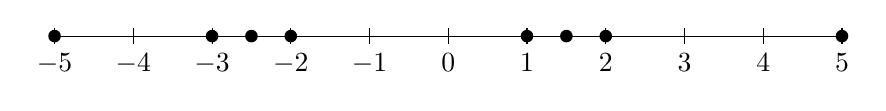
\begin{tikzpicture}
\draw (-5,0) -- (5,0);
		\foreach \i in {-5,-4,-3,-2,-1,0,1,2,3,4,5} % numbers on line
		{
		\draw (\i,0.1) -- + (0,-0.2) node[below] {$\i$};
		}
		\foreach \i in {-5, -3, -2.5, -2, 1, 1.5, 2, 5}% points on line
		\fill[black]  (\i,0) circle (0.8 mm);
\end{tikzpicture}
\caption{An example set of data points.} \label{fig:M1}
\end{figure}


As you could imagine, we could find a high degree polynomial to closely fit the data points. This is generally a bad idea as this complicated model overfits the given data and it is likely to generalize poorly on future data points. \\ 

\textbf{Mixture of Gaussian Distributions}

Instead, we could express the distribution of points as the superposition of a mixture of Gaussian distributions with weights. Recall the Gaussian distribution is a probability distribution defined by a mean $\mu$ and a variance $\sigma^2$.
\begin{equation}
\label{eq:transition1}
f(x \ \vert \ \mu , \sigma) = \frac{1}{\sqrt{2 \pi \sigma^2}} e^{-\frac{(x - \mu)^2}{2 \sigma^2}}
\end{equation}

Given $k$ Gaussian distributions, our model parameters would be $k$ weights $w_i$ such that $\sum_{i = 1}^k w_i = 1$ and the means and variances that define the Gaussian distributions $\{\ \mu_i, \ \sigma_i^2\ \ \}^k_{i = 1}$.
\begin{equation}
\label{eq:transition1}
data \ distribution \approx w_1GD_1 + w_2GD_2 + ... + w_kGD_k
\end{equation}

A bonus of this model is it gives us a way to generate a potentially infinite amount of synthetic data as we have a distribution. This brings up the question of does this distribution truly approximate the real distribution (assuming the data has a distribution)? An important observation is we have a discrete distribution as we have a finite number of data points. There is no distribution mass between the sampled points (in fig. 1 at $-4$ for example) and we don't have a true continuous distribution in the formal sense. \\

\textbf{Optimizing and Evaluating the Model}

Given $k$ Gaussian distributions and their weights, how do we optimize the model and evaluate how good a "fit" it is? For a single Gaussian distribution, the probability mass is $1$. A natural thing to do would be to take an interval of say $1/4$ the Gaussian distribution and this interval should contain $1/4th$ the points. This is an ok approach but it is hard to generalize. \\

Instead, we will frame optimization as a "likelihood" problem. That is, given a collection of parameters that define our model what is the likelihood this model generated the data?
\begin{equation}
\label{eq:transition1}
Pr[\mathcal{X} \ \vert \ f(\mu_i, \sigma_i, w_i, k)]
\end{equation}

\begin{figure}[H]
\centering
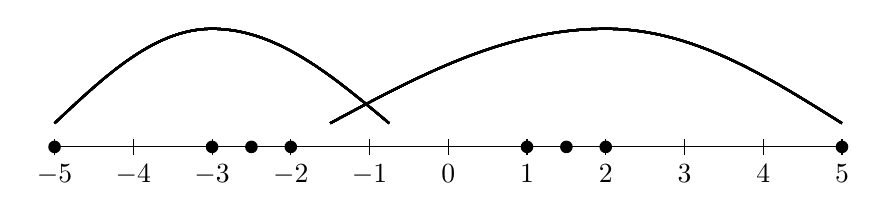
\begin{tikzpicture}
\draw (-5,0) -- (5,0);
		\foreach \i in {-5,-4,-3,-2,-1,0,1,2,3,4,5} % numbers on line
		{
		\draw (\i,0.1) -- + (0,-0.2) node[below] {$\i$};
		\draw[thick, black] (-1.5, 0.3) sin (2,1.5) cos (5,0.3);
		\draw[thick, black] (-5, 0.3) sin (-3, 1.5) cos (-0.75, 0.3);
		}
		\foreach \i in {-5, -3, -2.5, -2, 1, 1.5, 2, 5}% points on line
		\fill[black]  (\i,0) circle (0.8 mm);
\end{tikzpicture}
\caption{What is the likelihood the model generated these points?} \label{fig:M1}
\end{figure}

We want to maximize this likelihood and this is called the "maximum-likelihood" approach written as 
\begin{equation}
\label{eq:transition1}
\operatorname*{arg\,max}_\theta \ Pr[\mathcal{X} \ \vert \ \theta] = \prod_{i = 1}^n f(x_i \ \vert \ \theta) \ \ \ where \ \    \theta = \{\mu_i, \sigma_i, w_i, k\}
\end{equation}

We prefer to work with the natural logarithm of the likelihood function to avoid working with products. This is called the "log-likelihood" and we can now perform stochastic gradient descent to solve this optimization problem.
\begin{equation}
\label{eq:transition1}
\operatorname*{arg\,max}_\theta \ \sum_{i = 1}^n \ln f(x_i \ \vert \ \theta) \ \ \ where \ \    \theta = \{\mu_i, \sigma_i, w_i, k\}
\end{equation}

This is a traditional statistics approach to this problem. We guess a good model class and then find parameters in that class that maximize the log-likelihood. Unfortunately, finding the optimal parameters is NP-hard even in simple cases. To cope with this, we use a heuristic algorithm called the Expectation-maximization (EM) algorithm to approximate the optimal parameters. \\

While we can't prove this outside of very simple cases, this is similar to solving the Maximum likelihood estimation (MLE) problem. Unsupervised learning is often used as a preprocessor to supervised learning to learn something about the data by clustering it. \\

\textbf{Single Gaussian Distribution Example}

Even when trying to fit a single Gaussian distribution to a set of points, things are not simple and can be NP-hard. The probability of a given Gaussian distribution producing $N$ points is given as 
\begin{equation}
\label{eq:transition1}
Pr[\mathcal{X} \ \vert \ f(\mu, \sigma)] = \prod_{i = 1}^N \frac{1}{\sqrt{2 \pi \sigma^2}} e^{-\frac{(x_i - \mu)^2}{\sigma^2}} = \bigg(\frac{1}{2 \pi \sigma^2}\bigg)^{N/2} e^{-[\frac{(x_1 - \mu)^2}{\sigma^2} + ... + \frac{(x_N - \mu)^2}{\sigma^2}]}
\end{equation}

As such, we can frame maximizing the likelihood as a minimization problem
\begin{equation}
\label{eq:transition1}
\operatorname*{arg\,max}_{\mu, \sigma} Pr[\mathcal{X} \ \vert \ f(\mu, \sigma)] = \operatorname*{arg\,min}_{\mu, \sigma} \frac{\sum_{i = 1}^N (x_i - \mu)^2}{\sigma^2}
\end{equation}

That is, minimize the part of $e$'s power from eq. 6 that is in the brackets to maximize the entire expression. \\

Things only become more complicated when we consider a mixture of $k$ Gaussian distributions. As a heuristic, we try to minimize the objective from eq. 7 only for the nearest $\mu$ for each $x \in \mathcal{X}$.

\section{The \textit{k}-Means Problem}

To finish this lecture, we will introduce the \textit{k}-means problem. Given points $x_1, \ x_2, ... , \ x_N \in \mathcal{X}$ we want to find $\mu_1, \ \mu_2, ... , \ \mu_k \in \mathcal{X}^\prime$ ($\mu_i$ doesn't necessarily need to be a data point but a point from the same space) such that the following is minimized:
\begin{equation}
\label{eq:transition1}
\sum_{i = 1}^N (x_i - \mu_{c(i)})^2
\end{equation}

Where $c(i)$ is the index of the $\mu$ closest to point $x_i$. It turns out finding the optimal $\mu_1, \ \mu_2, ... , \ \mu_k$ solution is infeasible and NP-hard. Next lecture, we will take a closer look at this optimization problem and also an iterative algorithm (the k-means algorithm) to approximate a solution.
\end{document}
